\documentclass[compress]{beamer}
\usepackage{euscript,amsmath,amssymb,amsfonts,amsthm,epsfig,subfigure,color,graphicx,media9}
\usepackage[utf8]{inputenc}
\usepackage[french]{babel}
\usepackage[T1]{fontenc}
\usepackage{pgf,csquotes}
\usepackage{tikz}
\usetikzlibrary{fit,arrows,positioning}
\newsavebox{\mysavebox}

% \definecolor{blue}{rgb}{51,131,255}
%
%\usepackage[autolinebreaks,useliterate]{mcode}

% \usepackage{letltxmacro}
% \LetLtxMacro\olditemize\itemize
% \LetLtxMacro\oldenumerate\enumerate

\graphicspath{{figures/}}

\usepackage[doi=false,
            isbn=false,
            url=false,
            firstinits=true,
            bibstyle=authoryear,
            backend=biber,
            style=authoryear]{biblatex} %, backend=bibtex
\AtEveryCitekey{%\clearfield{title}
    \scriptsize
    \clearfield{note}
    \clearfield{pages}
    \clearfield{volume}%
    \clearfield{number}
    \clearlist{location}
    \clearlist{publisher}
    \clearname{editor}}
\renewcommand*{\multicitedelim}{\\}


\addbibresource{bib/strings.bib}
\addbibresource{bib/stringsShort.bib}
\addbibresource{bib/bib.bib}
\addbibresource{bib/references.bib}
\addbibresource{bib/journals.bib}
\addbibresource{bib/conferences.bib}
\addbibresource{bib/software.bib}

\usepackage{beamerthemedefault, multimedia, wasysym, amssymb, kpfonts}

\useoutertheme{smoothbars}
\useinnertheme[shadow=true]{rounded}
\setbeamercovered{transparent}
\setbeamertemplate{navigation symbols}{}
\setbeamertemplate{footline}[frame number]
\setbeamerfont{footline}{size=\fontsize{7}{11}\selectfont}
%\setbeamertemplate{itemize items}{$\multimapdotinv$}
%\setbeamertemplate{itemize items}{\textbf{$\strictfi$}}
\setbeamertemplate{enumerate items}[circle]
\setbeamertemplate{section in toc}[circle]
%\useoutertheme{infolines}
\setbeamercolor{block title}{bg=green}

\definecolor{violet}{rgb}{0.8, 0.6, 0.8}
\definecolor{green}{rgb}{0.8 ,.9, 0.8}
\definecolor{blue}{rgb}{0.3, 0 ,0.6}

\newcommand{\includesound}[1]{
\includemedia[
  addresource=#1,
  flashvars={
    source=#1
   &autoPlay=true
  }
]{\structure{
\includegraphics[keepaspectratio,width=.5cm]{figures/play}}}{APlayer.swf}
}

% footnote without numbers
\let\oldfootnote\footnote
\renewcommand\footnote[1]{\let\thefootnote\relax%
\oldfootnote{#1}}

\newrobustcmd*{\footfullcitenomark}{%
  \AtNextCite{%
    \let\thefootnote\relax
    \let\mkbibfootnote\mkbibfootnotetext}%
  \footfullcite}

  \defbeamertemplate*{footnotetext}{default}{%
  %\parindent 1em\noindent%
  \raggedright
  %\hbox to 1.8em{\hfil\insertfootnotemark}%
  \insertfootnotetext\par}

\newrobustcmd*{\footfullcitenomarkleft}{%
  \AtNextCite{%
    \setbeamertemplate{footnote}{\usebeamertemplate{footnotetext}}%
    \let\mkbibfootnote\mkbibfootnotetext}%
  \footfullcite}

% title, url, authors, extensions
\newcommand\citenote[4]{\footnote{#3 \href{#2}{\structure{#1}} #4}}


\setbeamertemplate{itemize item}{\textrm{--}}

% \defbeamertemplate{description item}{align left}{\insertdescriptionitem\hfill}
% \setbeamertemplate{description item}[align left]

%\usecolortheme[named=purple]{structure}

\title[]{\LARGE \bf Soutenance d'habilitation à diriger les recherches}

\subtitle{\og Modélisation Long-Terme de Signaux Sonores \fg}

\author{Mathieu Lagrange}

\institute[]
{
\begin{minipage}{.5\columnwidth}
  \tiny
\begin{description}
\item[Frédéric Bimbot] Directeur de Recherche CNRS, IRISA, Rennes
\item[Alain de Cheveigné] Directeur de Recherche CNRS, ENS Paris
\item[Béatrice Daille] Professeur, LS2N, Nantes
\item[Patrick Flandrin] Directeur de Recherche CNRS, ENS Lyon
\item[Stéphane Mallat] Professeur, Collège de France
\end{description}
\end{minipage}
\begin{minipage}{.4\columnwidth}
  \centering
  
\includegraphics[height=2cm]{figures/logoLs2n}\\
  \includesound{sounds/hello.mp3}
\end{minipage}

% 
\includegraphics[height=1.5cm]{figures/logoEcn}
% 
\includegraphics[height=1.5cm]{figures/logoCnrs}
}

\date[]{14 Novembre 2019}

\logo{
\includegraphics[height=.6cm]{figures/logoCnrs}}

\begin{document}

\tikzstyle{mystyle}=[
nonterminal/.append style={join=by ->},
tip/.style={->,shorten >=1pt},every join/.style={rounded corners},
terminal/.style={
% The shape:
rectangle,minimum size=6mm,rounded corners=1mm,
% The rest
very thick,draw=black!50,
top color=white,bottom color=black!10,
font=\ttfamily},
point/.style={circle,fill=black,minimum size=2pt},
%every node/.style=draw,
line/.style ={draw, thick, -latex',shorten
  >=2pt}]

  \AtBeginSection[]{
    \begin{frame}
    \vfill
    \centering
    \begin{beamercolorbox}[sep=8pt,center,shadow=true,rounded=true]{title}
      \huge \bf
      \secname\par%
    \end{beamercolorbox}
    \vfill
    \end{frame}
  }

% Update itemize to have a default overlay
%\renewcommand{\itemize}[1][<+(1)->]{\olditemize[#1]}
%\renewcommand{\enumerate}[1][<+(1)->]{\oldenumerate[#1]}

%\includeonlyframes{current}

\frame{\titlepage \thispagestyle{empty}}

% show section lists
\begin{frame}{Agenda} \tableofcontents \end{frame} % [pausesections]

\section[Cv]{Curriculum Vit\ae}\begin{frame}{Statut}
\begin{block}{Chargé de recherche CNRS classe normale}
\structure{2009} : recrutement par la commission interdisciplinaire (CID) 44 : \og Cognition, langage, traitement de l’information, systèmes \fg \\
\structure{2012} : rattachement à la section 07 : \og Sciences de l'information \fg
\end{block}
\begin{block}{Qualifications CNU}
\structure{section 27} : \og Informatique \fg \\
\structure{section 61} : \og Génie informatique, automatique et traitement du signal \fg
\end{block}
\end{frame}

\begin{frame}{Diplômes}
\begin{block}{Master Informatique (2001)}
\structure{Intitulé} : \og Accélération de la synthèse sonore \fg \\
\structure{Encadrement} : Sylvain Marchand, Robert Strandh \\
\structure{Lieu de soutenance} : Université de Bordeaux 1
\end{block}
\begin{block}{Doctorat Informatique (2004)}
\structure{Intitulé}: \og Modélisation sinusoïdale des signaux polyphoniques \fg \\
\structure{Direction}: Myriam Desainte-Catherine \\
\structure{Encadrement}: Sylvain Marchand et Jean-Bernard Rault \\
\structure{Lieu de soutenance}: Université de Bordeaux 1
\end{block}
\end{frame}


\begin{frame}{Carrière}
\small
    \begin{tabular}{ll}
  2001-4 & {\bf Doctorant Université Bordeaux 1} \\
  &  Ingénieur de Recherche  à France Télécom R\&D Rennes \\
  & TECH/IRIS (équipe codage et multimédia) \\
  2004-5 & {\bf Enseignant chercheur (ATER)} au LaBRI (U. Bx. 1)  \\
  2005-6 & {\bf Enseignant chercheur (ATER)}  à l'Enseirb (U. Bx. 1) \\
  2006-7 & {\bf Post-doctorant} au sein du département d'informatique \\
  &  Université de Victoria, BC, Canada \\
 2007-8 &  {\bf Post-doctorant} au sein du département "Music Technology"  \\
  &  Université de McGill, QC, Canada \\
 2008-9 &  {\bf Post-doctorant} au sein de  l'équipe    \\
  & \og Acoustique Audio et Ondes \fg, Télécom ParisTech \\
 2009-13 &  {\bf Chercheur CNRS} au sein de l'équipe Analyse / Synthèse  \\
  & Ircam (Umr 9912), Paris \\
 2013- -- &  {\bf Chercheur CNRS} au sein de l'équipe \\
 & Signal, Images et Son (Sims)  \\
  & Ls2n (Umr 6004), Ecole Centrale de Nantes \\
\end{tabular}
\end{frame}


\begin{frame}{Contributions}

\begin{block}{Indices bibliométriques}
\begin{itemize}
\item 21 revues internationales à comité de lecture
\item 62 conférences internationales à comité de lecture
\item citations: 1784 (source Google Scholar, Oct. 2019)
\item indice h: 19 (source Google Scholar, Oct. 2019)
\end{itemize}
\end{block}
\begin{block}{Responsabilités}
\begin{itemize}
\item relecteur pour 8 revues et 12 conférences du domaine
\item adjoint à la direction de l'équipe SIMS
\item membre du comité directeur de l'association sportive de l'\'Ecole Centrale de Nantes
\end{itemize}
\end{block}
\end{frame}

\begin{frame}{Enseignement (h eq. TD)}
\begin{itemize}
  \item \structure{Cursus Ingénieur} :
  \begin{itemize}
    \item apprentissage automatique pour le traitement du signal audionumérique (24h)
    \item musique numérique (15h)
  \end{itemize}
  \item \structure{Master 2} : apprentissage automatique (9h)
  \item \structure{Formation doctorale} : méthodologie de la recherche (18h)
\end{itemize}
\end{frame}

\begin{frame}{Encadrement}
\begin{itemize}
  \item \structure{Rémi Foucard} (2010 - 2013): \og Fusion multi-niveaux par boosting pour le tagging automatique \fg
  \item \structure{Grégoire Lafay} (2013 - 2016): \og Simulation de scènes sonores environnementales : application à l'analyse sensorielle et à l'analyse automatique \fg
  \item \structure{Jean-Rémy Gloaguen} (2015 - 2018): \og Estimation du niveau sonore de sources d'intérêt au sein de mélanges sonores urbains : application au trafic routier \fg
  \item \structure{Félix Gontier} (2017 - --): \og Modélisation de signaux sonores par approches neuronales profondes \fg
  \item \structure{Tom Souaille} (2019 - --): \og Conception interactive en design sonore \fg
\end{itemize}
\end{frame}

\section[Problématiques]{Problématiques en traitement du signal audio-numérique} \begin{frame}{Traitement du signal audio-numérique}
\begin{block}{Besoins et problématiques associées}
\structure{Transmission}: Codage \\
\structure{Indexation}: Recherche d'Information (IR) \\
\structure{Création}: Synthèse sonore
\end{block}
\begin{block}{Domaines d'application}
\begin{itemize}
\item Musique
\item Sons environnementaux
\end{itemize}
\end{block}
\end{frame}


\begin{frame}{Besoins de compacité}
\begin{block}{Verrou}
\begin{itemize}
\item une seconde de son : $$ x \in \mathbb{R}^{44100}$$
\item besoin d'une représentation plus \alert{compacte}
\end{itemize}
\end{block}
\begin{block}{Types de compacité}
\structure{Codage}: compacité signal \\ % ($ y \in \mathbb{R}^{5000}$) \\
\structure{Recherche d'information}: compacité sémantique \\ %  ($ y \in \mathbb{N}^{100}$) \\
\structure{Synthèse}: compacité \alert{\og} \structure{signalo-sémantique} \alert{\fg} \\ %  ($ y \in \mathbb{R}^{100}$)
\end{block}
\end{frame}

\begin{frame}{Codage compressif par transformée}
$$y = C(x) | \tilde{x} = C^{-1}(y), P_e(x) \simeq P_e(\tilde{x})$$
\begin{itemize}
\item $C$ : Quantification adaptative d'un équivalent de la Transformée de Fourier à Court Terme (TFCT)
\item $P_e$ : Modélisation de la sensibilité aux déformations de la membrane basilaire\footfullcitenomarkleft{zwicker2013psychoacoustics}
\end{itemize}
\end{frame}

\begin{frame}{Transformée de Fourier à Court Terme (TFCT)}
$$ f[m, t] = \sum_{n = - \infty}^{\infty} x[n] w[n-t] \mathrm{e}^{\frac{-2 \mathrm{j}  \pi m n}{N}} $$

\begin{description}
\item[$x$]: signal temporel
\item[$f$]: composantes fréquentielles (paniers, bins, ...)
\item[$w$]: fenêtre
\end{description}
\footfullcitenomarkleft{lostanlen2019fourier}
\end{frame}

\begin{frame}{Spectrogramme : $|f[m, t]|$}
\begin{center}
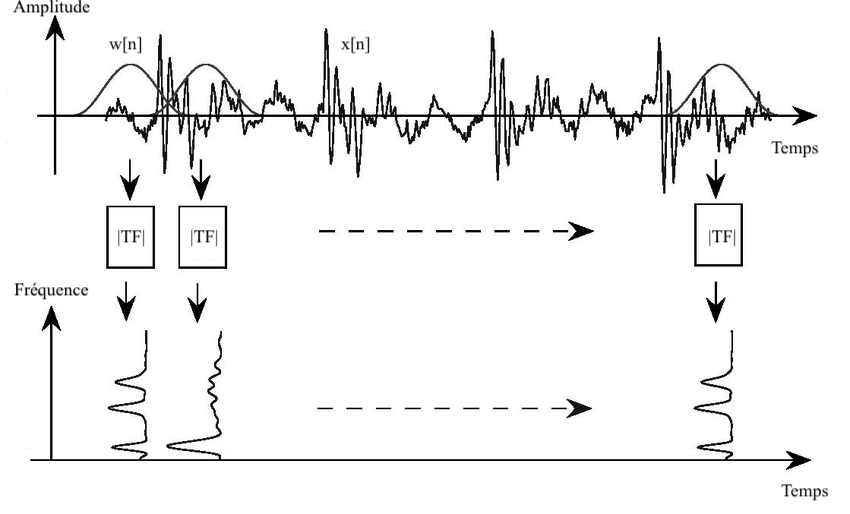
\includegraphics[width=.8\columnwidth]{figures/tfct} \\
\end{center}
\end{frame}

\begin{frame}{Spectrogramme}
\begin{center}
\only<1>{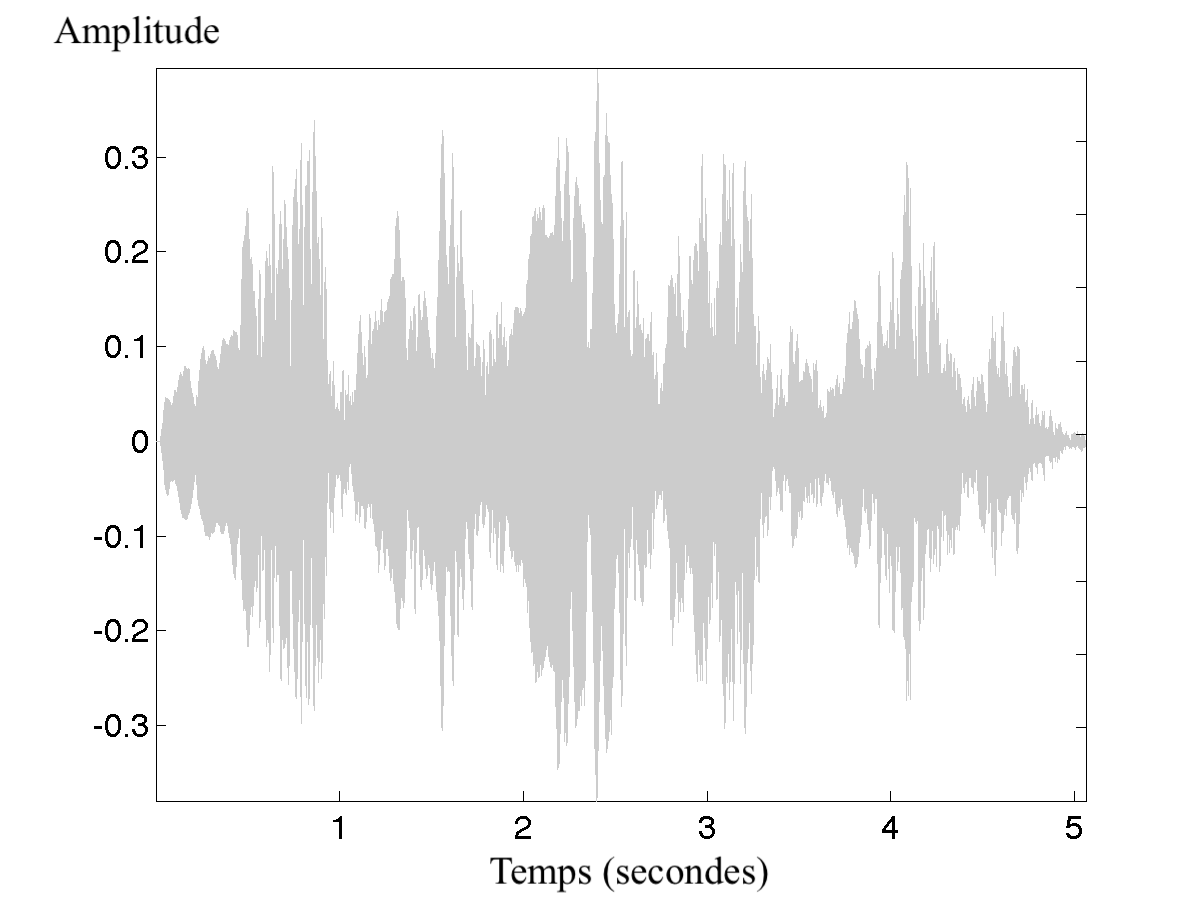
\includegraphics[width=.8\columnwidth]{figures/soloTime}}
\only<2>{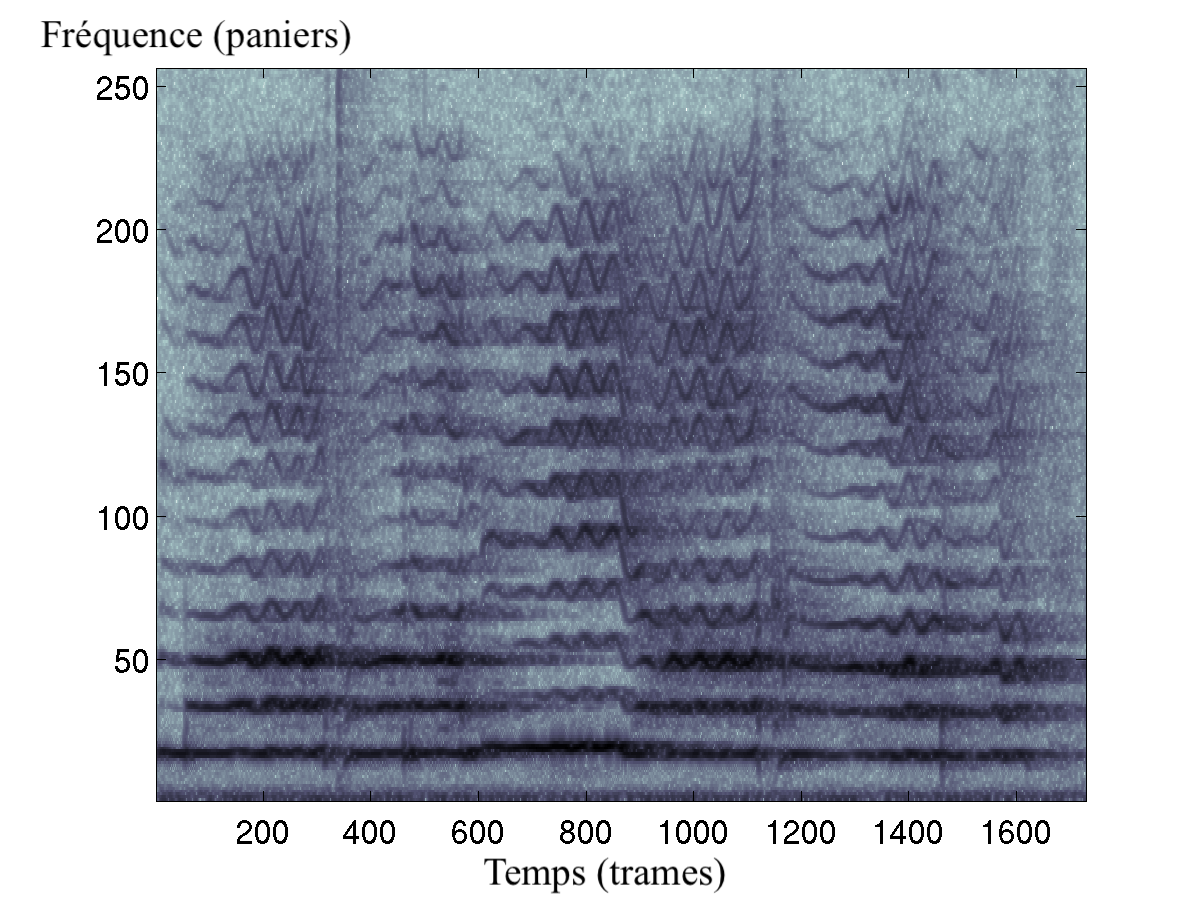
\includegraphics[width=1.1\columnwidth]{figures/soloSpec}}

\includesound{sounds/solo.mp3}
\end{center}
\end{frame}

\begin{frame}{Typologie des évènements sonores}
  \begin{tabular}{l|cc}
    & \multicolumn{2}{c}{structure} \\
  \structure{sons}  & horizontale & verticale \\
    \hline
    \structure{de parole} & sons voisés & sons plosifs  \\
    & <a>, <o> &  <pe>, <qe> \\
    \structure{d'animaux} & chants & clics  \\
    \structure{musicaux} & chant lyrique & percussions \\
    \structure{mécaniques} & ventilation & marteau piqueur \\
    \structure{environnementaux} & vent & gouttes de pluie \\
  \end{tabular}
\end{frame}

\begin{frame}{Compromis temps/fréquence}
	$\hookrightarrow{}$ mitiger cette contrainte imposée par l'approche court-terme par l'utilisation d'\alert{\textit{a priori}} sur les sources d'intérêt.
\end{frame}

\section[CASA]{Analyse computationnelle de scènes auditives (CASA)} \begin{frame}{\alert{Tâche} : Codage par transformée}
$$y = C(x) | \tilde{x} = C^{-1}(y), P_e(x) \simeq P_e(\tilde{x})$$
\begin{itemize}
\item $C$ : Quantification adaptative d'un équivalent de la Transformée de Fourier à Court Terme (TFCT)
\item $P_e$ : Modélisation de la sensibilité aux déformations de la membrane basilaire\footfullcitenomarkleft{zwicker2013psychoacoustics}
\end{itemize}
\end{frame}

\begin{frame}{Transformée de Fourier à Court Terme (TFCT)}
$$ X[m, t] = \sum_{n = - \infty}^{\infty} x[n] w[n-t] \mathrm{e}^{\frac{-2 \mathrm{j}  \pi m n}{N}} $$

\begin{description}
\item[$x$]: signal temporel
\item[$X$]: composantes fréquentielles (paniers, bins, ...)
\item[$w$]: fenêtre
\end{description}
\end{frame}

\begin{frame}{Spectrogramme : $|X[m, t]|$}
\begin{center}
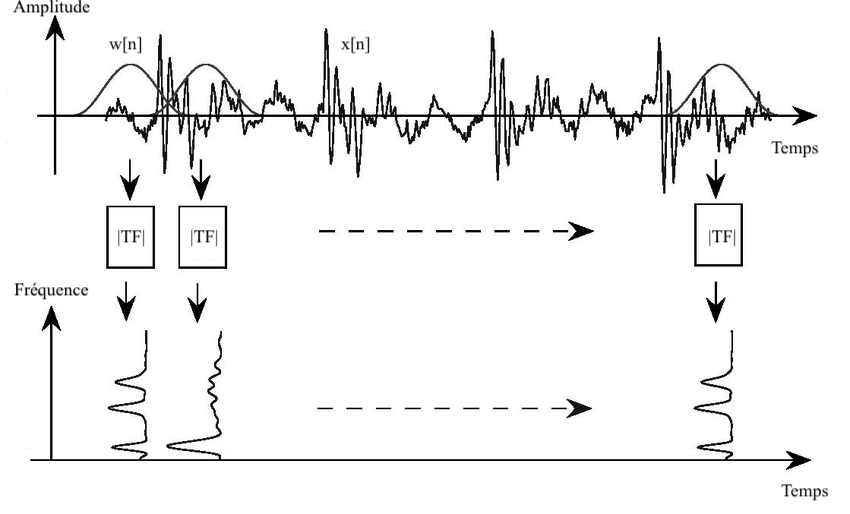
\includegraphics[width=.8\columnwidth]{figures/tfct} \\
\end{center}
\end{frame}

\begin{frame}{Spectrogramme}
\begin{center}
\only<1>{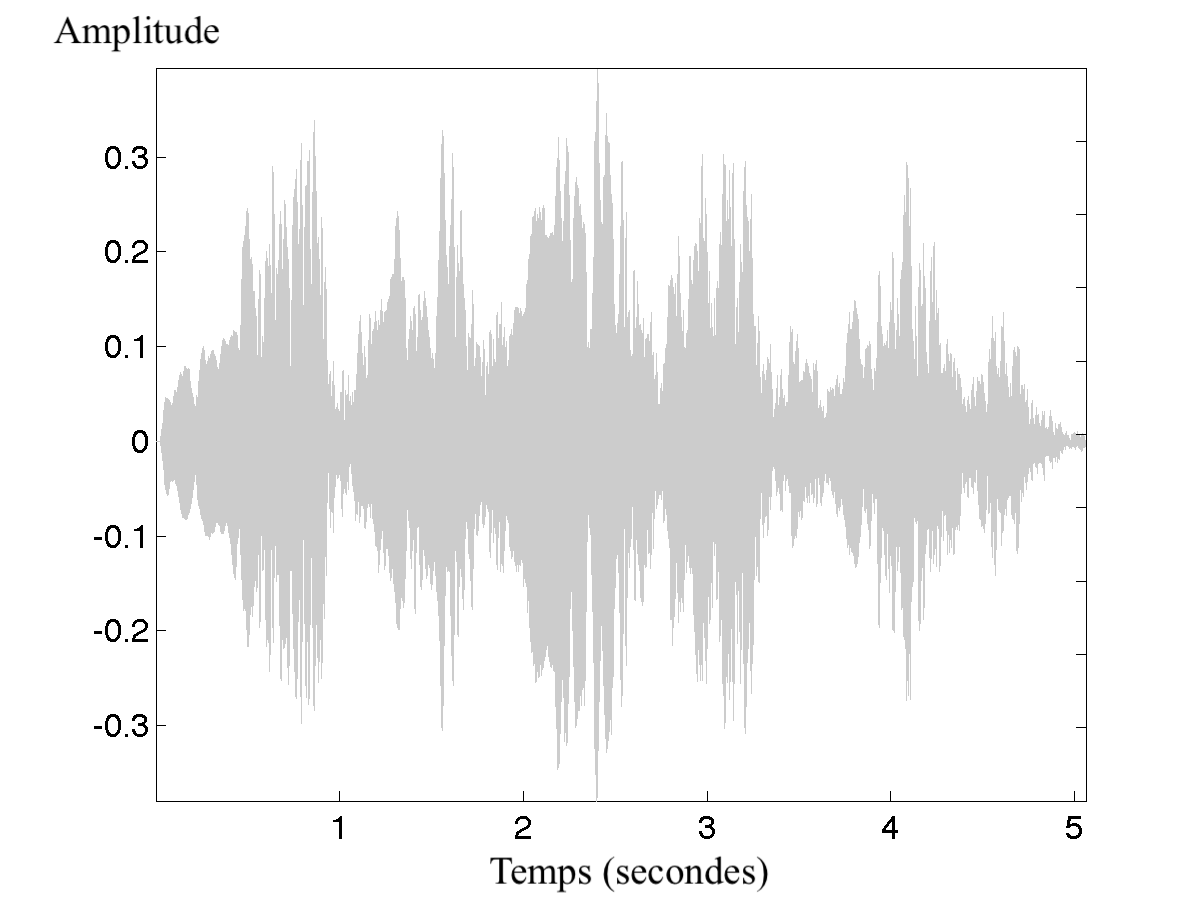
\includegraphics[width=.8\columnwidth]{figures/soloTime}}
\only<2>{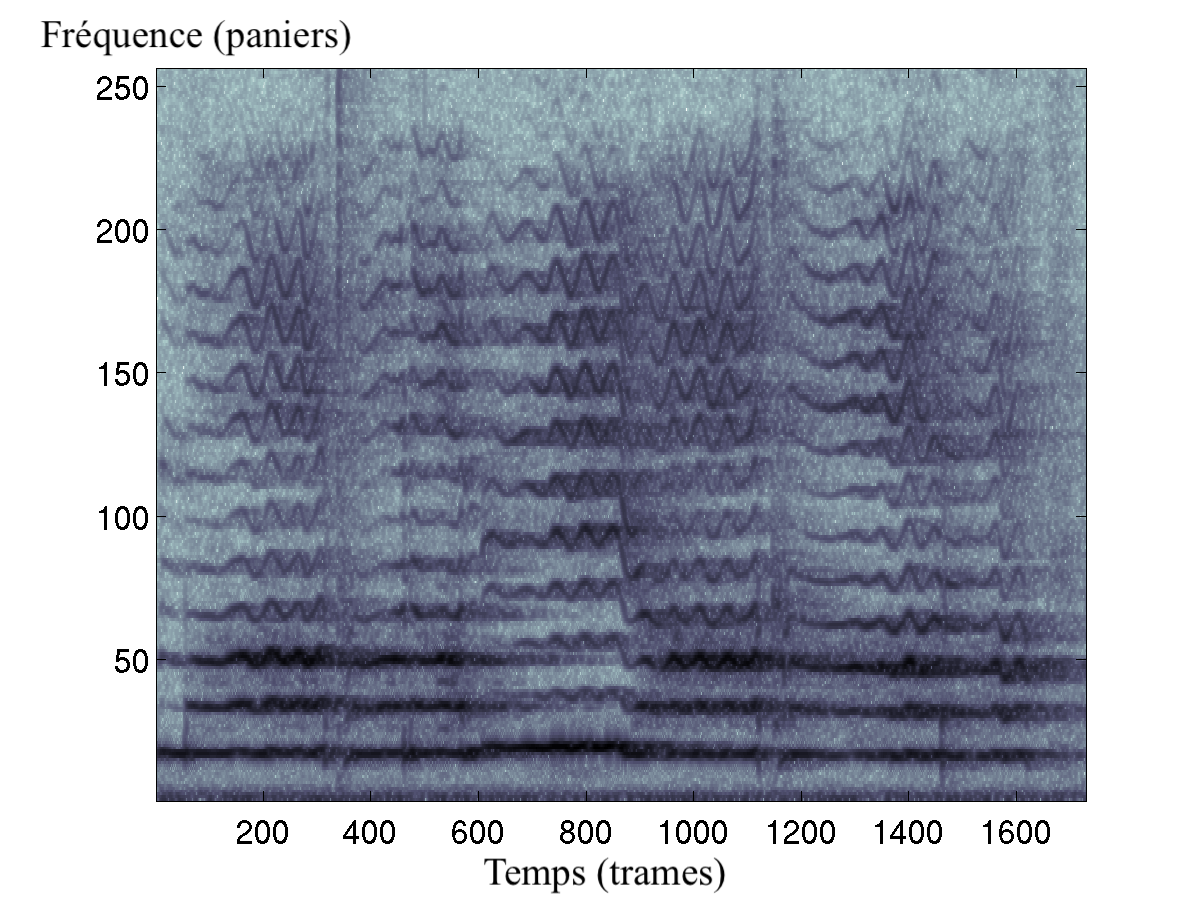
\includegraphics[width=.8\columnwidth]{figures/soloSpec}}

\includesound{sounds/solo.wav}
\end{center}
\end{frame}

\begin{frame}{Typologie des évènements sonores}
  \begin{tabular}{l|cc}
    & \multicolumn{2}{c}{structure} \\
  \structure{sons}  & horizontale & verticale \\
    \hline
    \structure{de parole} & sons voisés & sons plosifs  \\
    & <a>, <o> &  <pe>, <qe> \\
    \structure{d'animaux} & chants & clics  \\
    \structure{musicaux} & chant lyrique & percussions \\
    \structure{mécaniques} & ventilation & marteau piqueur \\
    \structure{environnementaux} & vent & gouttes de pluie \\
  \end{tabular}
\end{frame}

\begin{frame}{Compromis temps/fréquence}
	$\hookrightarrow{}$ mitiger cette contrainte imposée par l'approche court-terme par l'utilisation d'\alert{\textit{a priori}} sur les sources d'intérêt.
\end{frame}

\begin{frame}{Analyse de Scènes Auditives Computationelle (CASA)}
L'ASA\footfullcitenomarkleft{bregman1994auditory} étudie l'ensemble de traitements perceptifs permettant
\begin{itemize}
\item d'isoler les informations émanant d'\structure{entités} sonores distinctes,
\item de les organiser en un tout cohérent.
\item à l'aide de processus \structure{\og primitifs \fg} et \structure{\og séquentiels \fg}.
\end{itemize}
L'Analyse de Scènes Auditives Computationnelle (CASA)\footfullcitenomarkleft{wang2016casa} se propose de mettre en \oe~euvre ces critères pour inférer une organisation perceptuellement valide de la scène sonore.
\end{frame}

\begin{frame}{Processus ASA \og primitifs \fg}
\begin{description}
\item[\alert<2>{continuité}] : les propriétés d'un son isolé tendent à se modifier lentement et de façon continue
\item[harmonicité] : lorsqu'un corps sonore vibre à une période répétée, ses vibrations donnent naissance à un motif acoustique dont les fréquences des composants sont des multiples d'une même fréquence fondamentale;
\item[...]
\end{description}
\end{frame}

\begin{frame}{Modèle sinusoïdal à long terme}
\only<1>{
$$
x[n]=\sum_{l=1}^{L} a_{l}[n] \sin \left(\frac{2 \pi}{F_{s}} f_{l}[n] \cdot n + \Phi_k \right)
$$
$a_{l}[n]$ et $f_{l}[n]$ sont des signaux contrôlant respectivement l'amplitude et la phase des $L$ oscillateurs composant le modèle.
}
\begin{center}
\only<3>{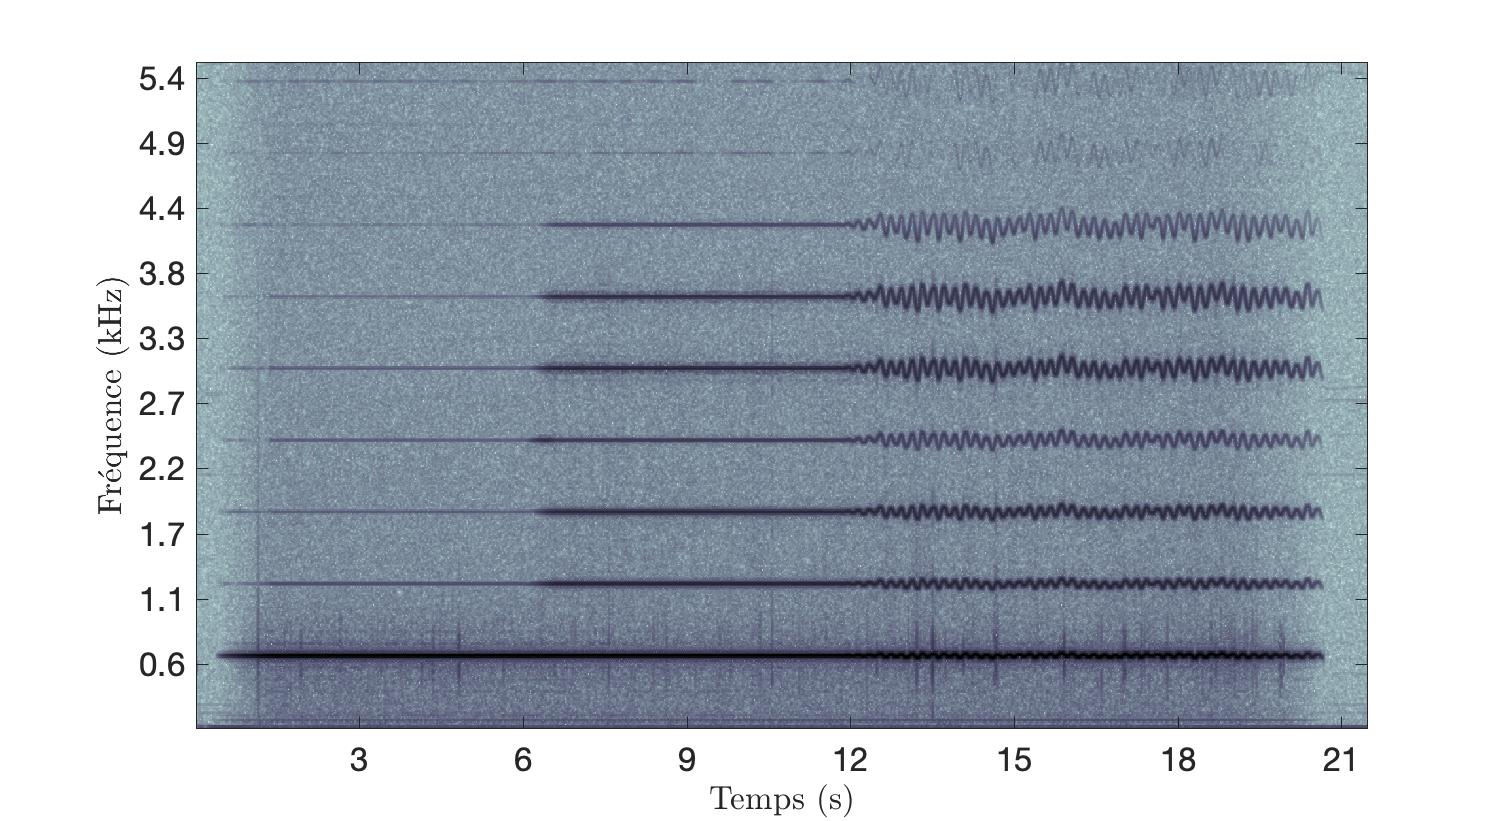
\includegraphics[width=1\columnwidth]{figures/asaSpec}}
\only<2->{\includesound{sounds/asa.wav} John Chowning}
\end{center}
%http://webpages.mcgill.ca/staff/Group2/abregm1/web/snd/Track24.mp3
\end{frame}

\begin{frame}{Procédé d'analyse de signaux sonores}
\begin{center}
\begin{tikzpicture}[mystyle]

  \matrix [column sep=10mm,row sep=5mm]
{
\node (i1) {}; \\
\node [terminal] (i2) {tfct}; \\
\node [terminal] (i3) {sélection de pics}; \\
\node [terminal] (i4) {suivi de partiel}; \\
\node  (i5) {}; \\
};

\begin{scope}[every path/.style=line]
  \path (i1) -- node [right] {signal} (i2);
  \path (i2) -- node [right] {spectrogramme} (i3);
  \path (i3) -- node [right] {atomes } (i4);
  \path (i4) -- node [right] {partiels} (i5);
\end{scope}
\end{tikzpicture}
\end{center}
\end{frame}

\begin{frame}{Atomes temps/fréquences}
\begin{center}
 \only<1>{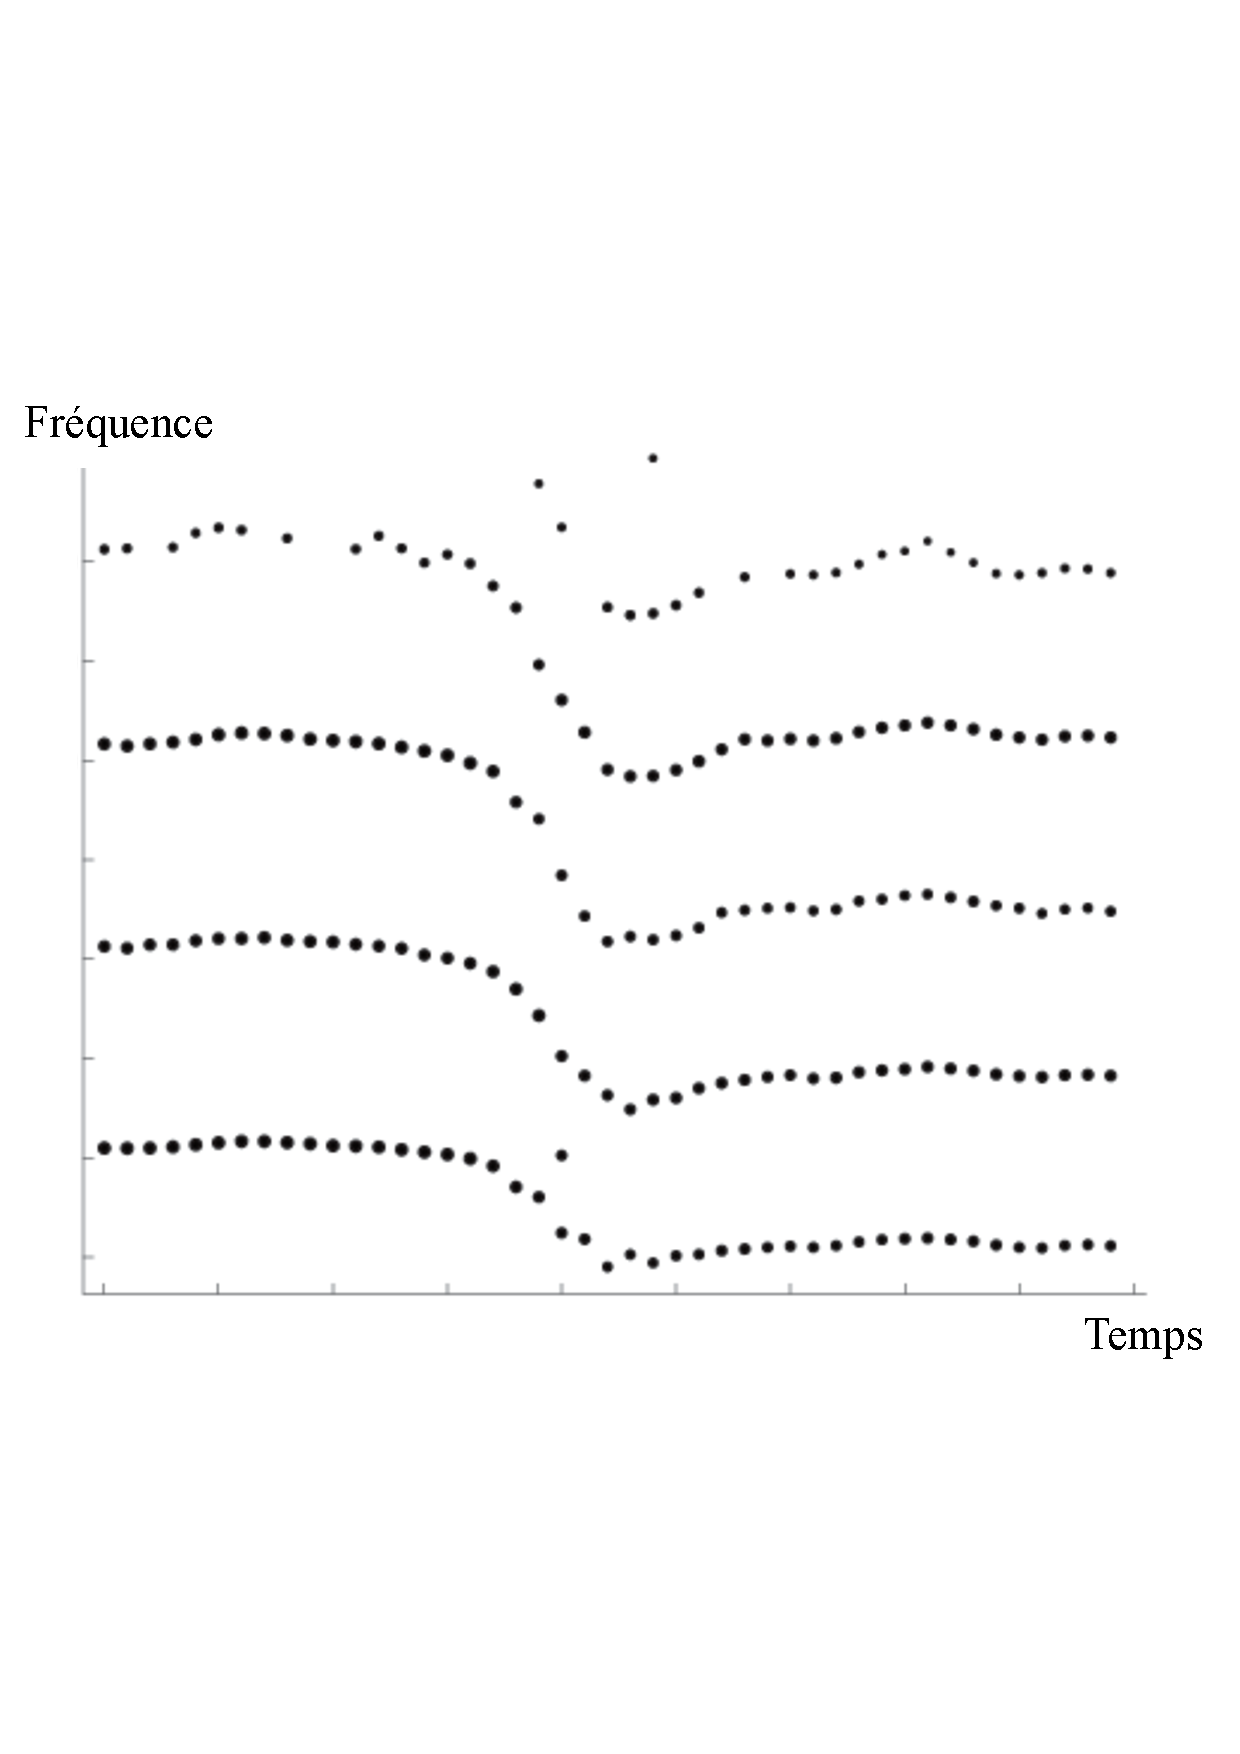
\includegraphics[width=.6\textwidth]{voice_1024_512xp} \\
 Taille de fenêtre : \structure{23} ms, pas d'avancement 10 ms.}
 \only<2>{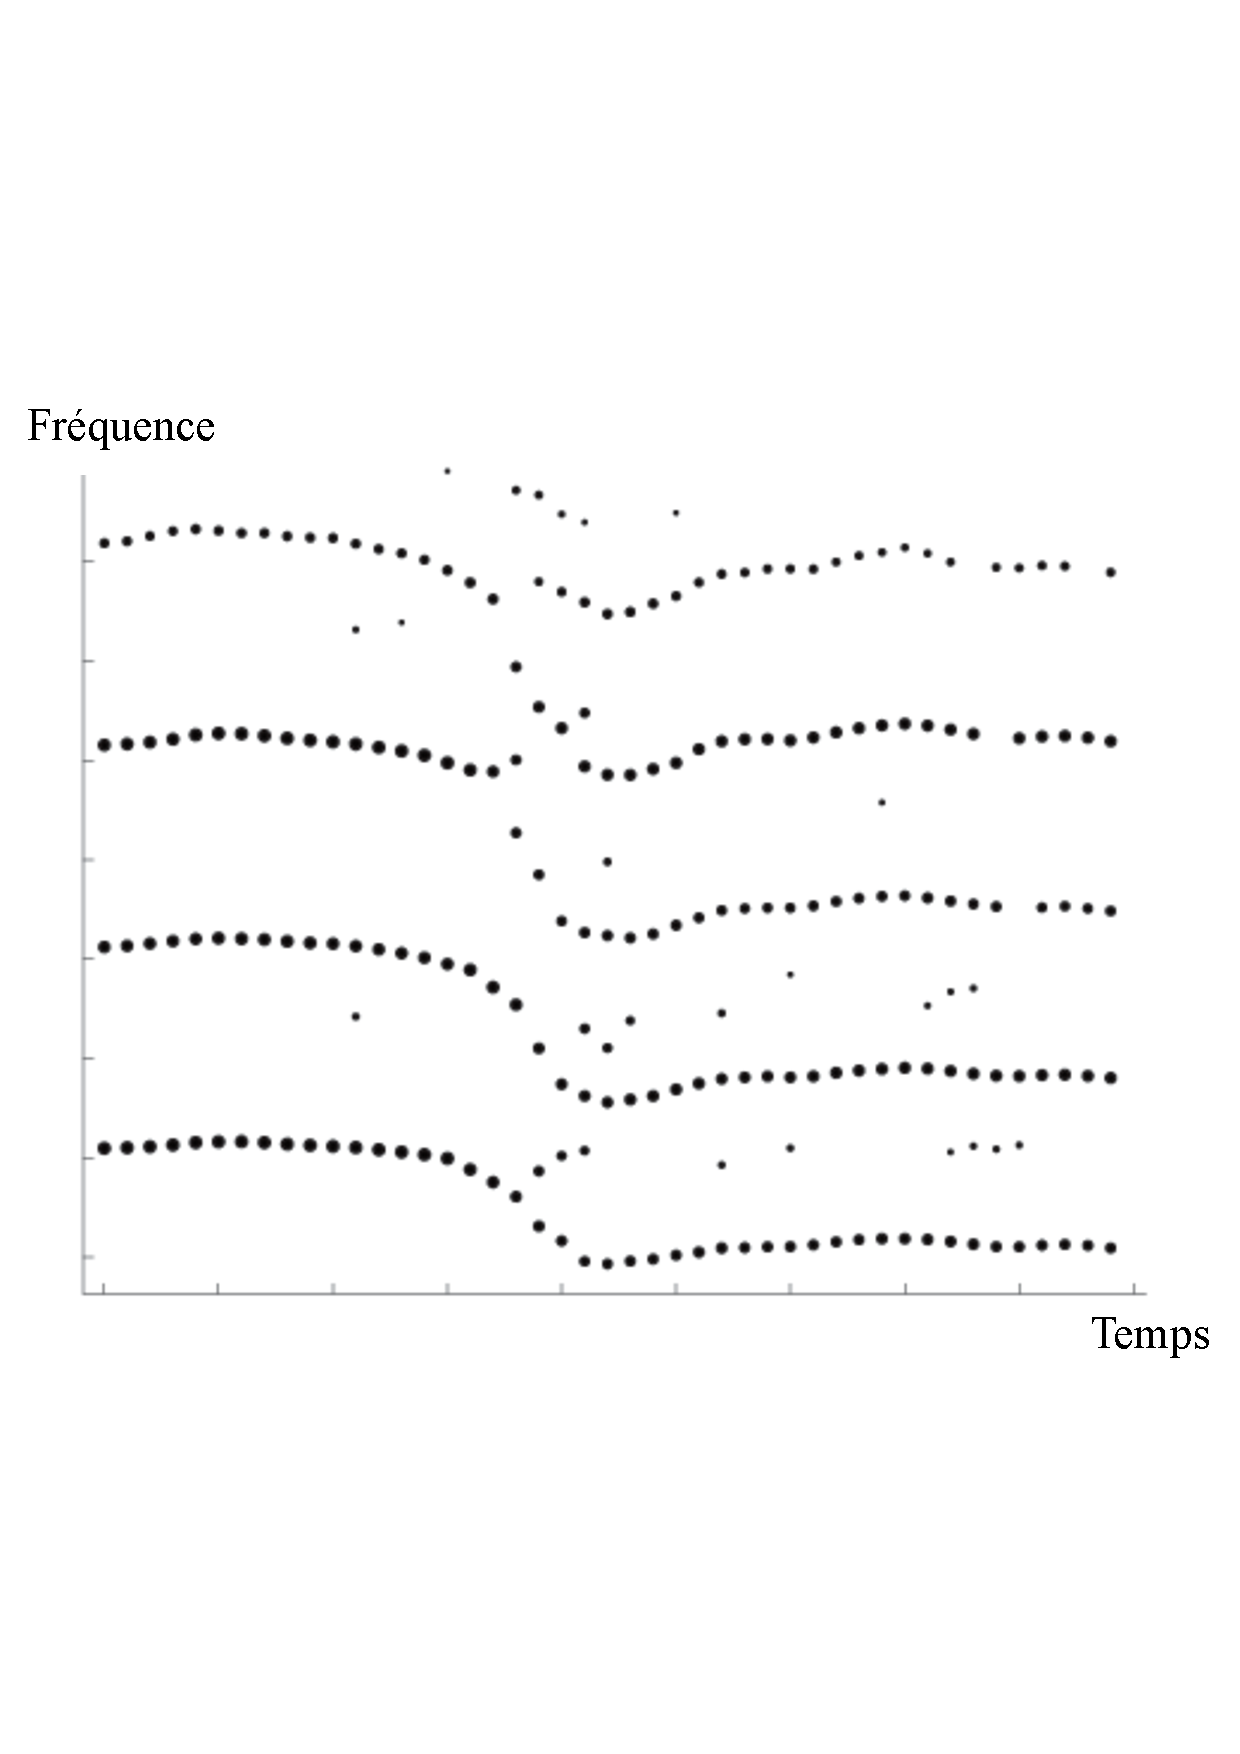
\includegraphics[width=.6\textwidth]{voice_2048_512xp} \\
 Taille de fenêtre : \structure{46} ms, pas d'avancement 10 ms.}
 \only<3>{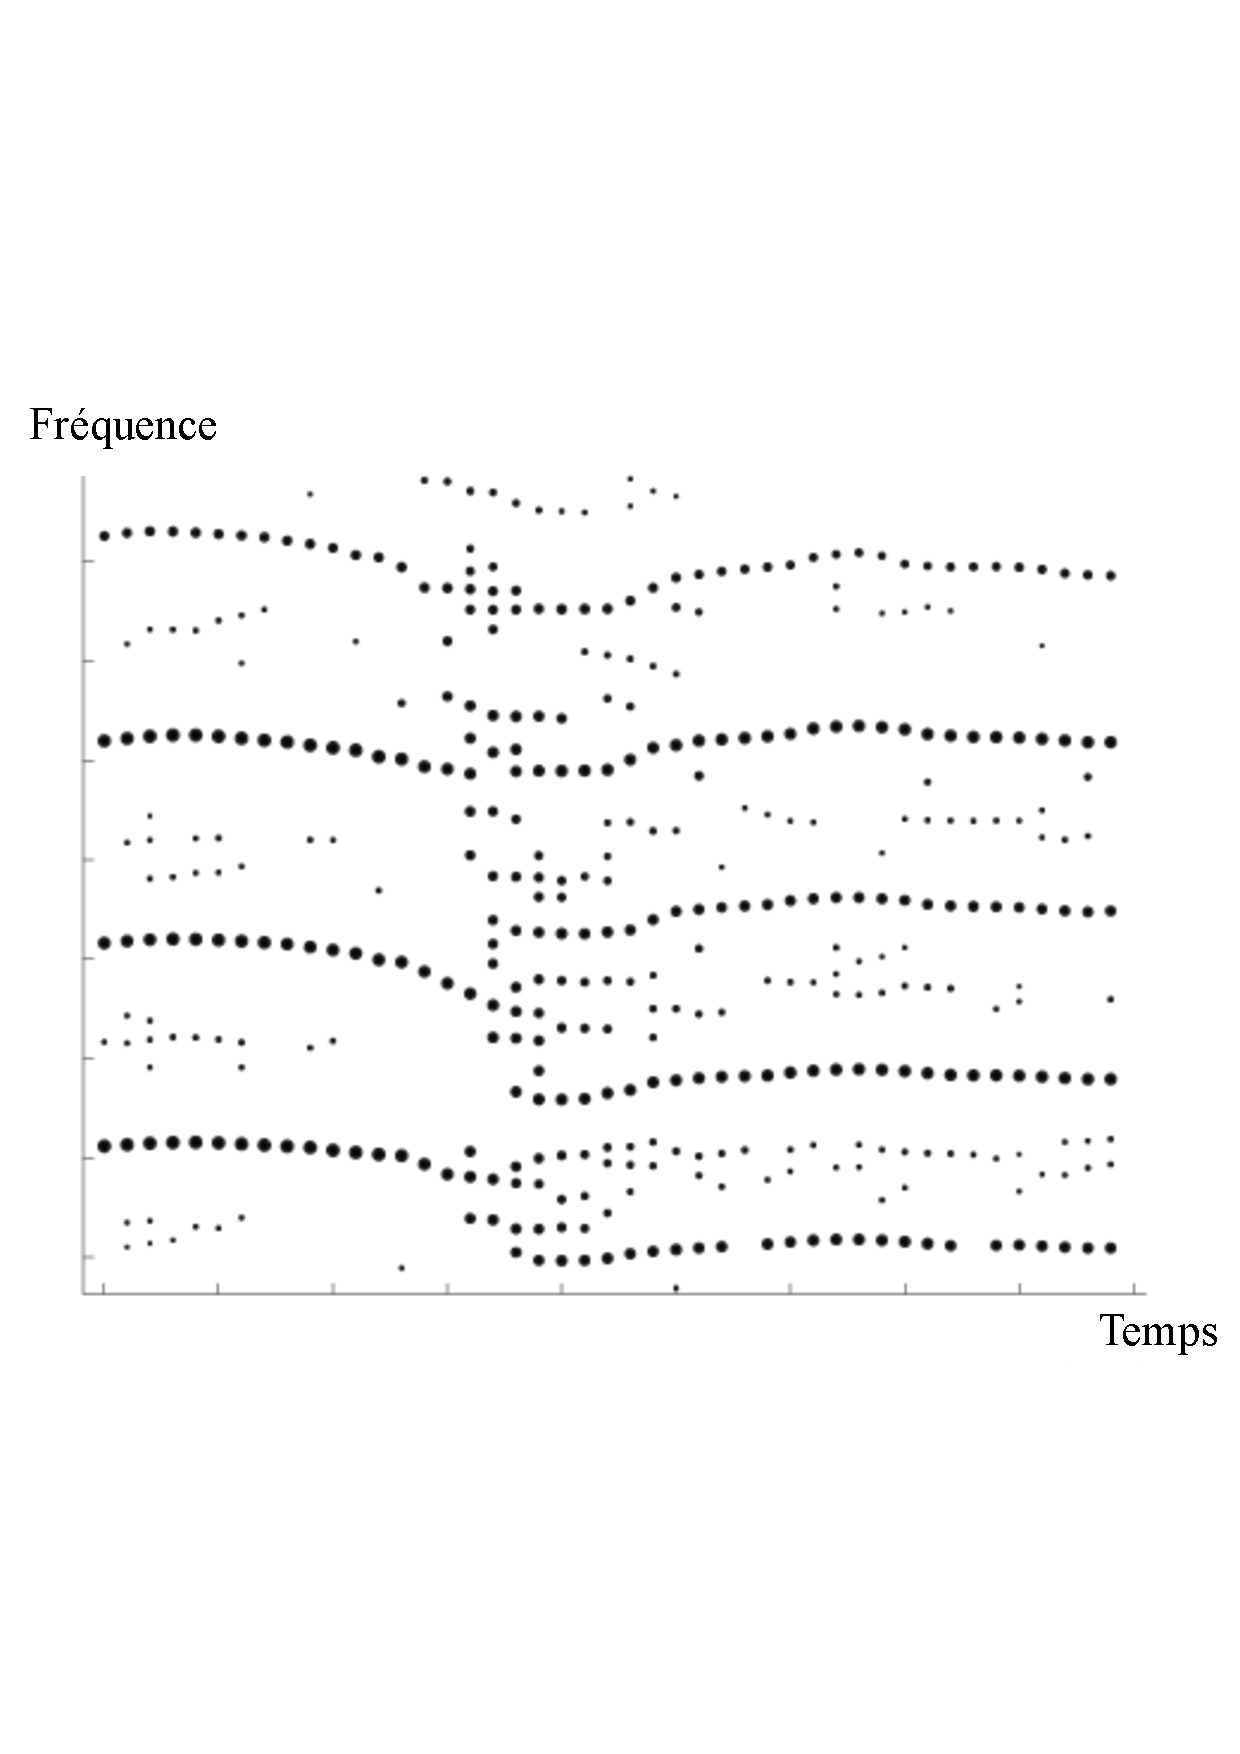
\includegraphics[width=.6\textwidth]{voice_4096_512xp} \\
 Taille de fenêtre : \structure{92} ms, pas d'avancement 10 ms.}
\end{center}
\end{frame}

\begin{frame}{Algorithme de suivi amélioré\footfullcitenomarkleft{lagrangeTaslp06}}
\begin{center}
  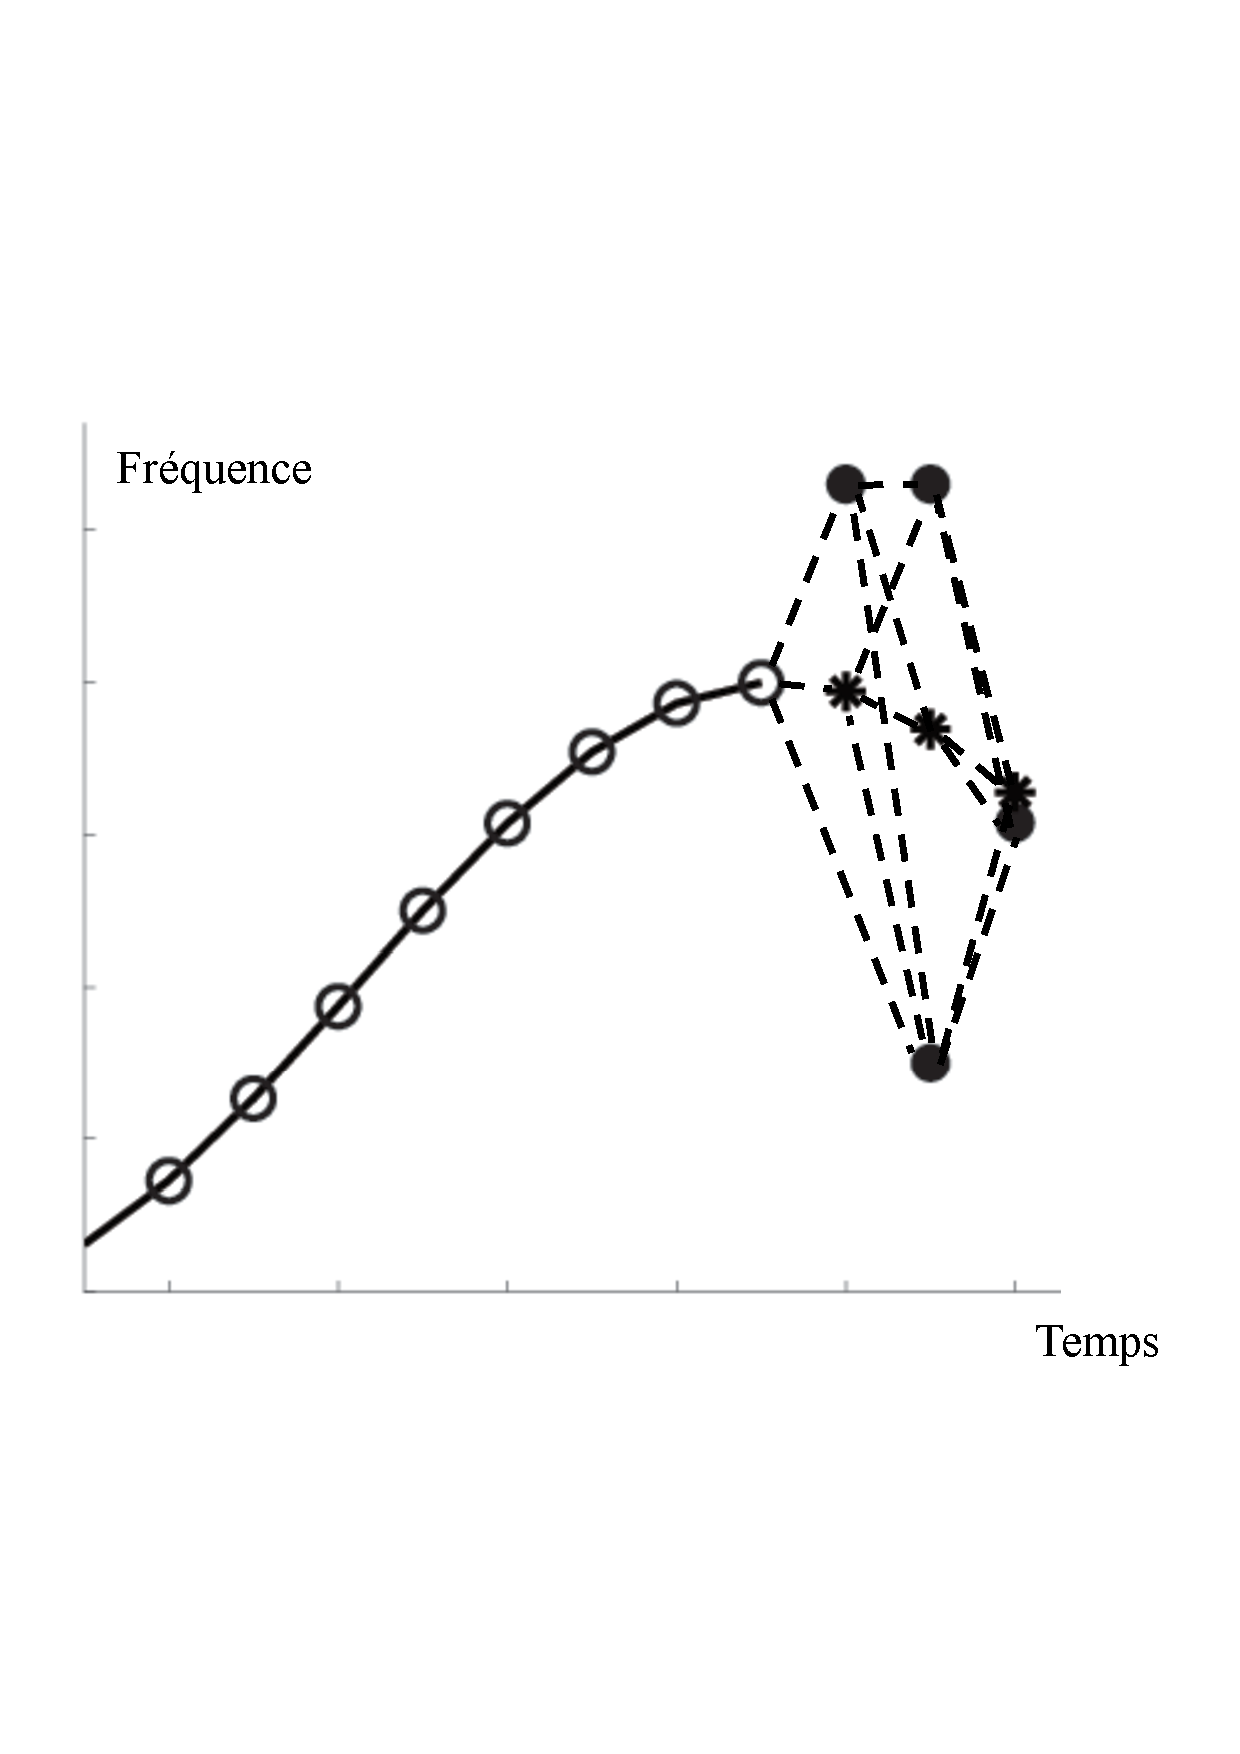
\includegraphics[width=.35\textwidth]{trackingxp2xp2}
\end{center}
  \begin{enumerate}
      \item Prédiction auto-régressive de l'évolution des paramètres de fréquence et d'amplitude
      \item Sélection des continuations engendrant le moins de hautes fréquences
  \end{enumerate}
\end{frame}

%todo minipage

\begin{frame}{Processus ASA \og primitifs \fg}
\begin{description}
\item[\alert{continuité}] : les propriétés d'un son isolé tendent à se modifier lentement et de façon continue
\item[\alert{harmonicité}] : lorsqu'un corps sonore vibre à une période répétée, ses vibrations donnent naissance à un motif acoustique dont les fréquences des composants sont des multiples d'une même fréquence fondamentale;
\item[...]
\end{description}
\end{frame}

\begin{frame}{Algorithme par coupures normalisées de graphes}
\begin{center}
 \only<1>{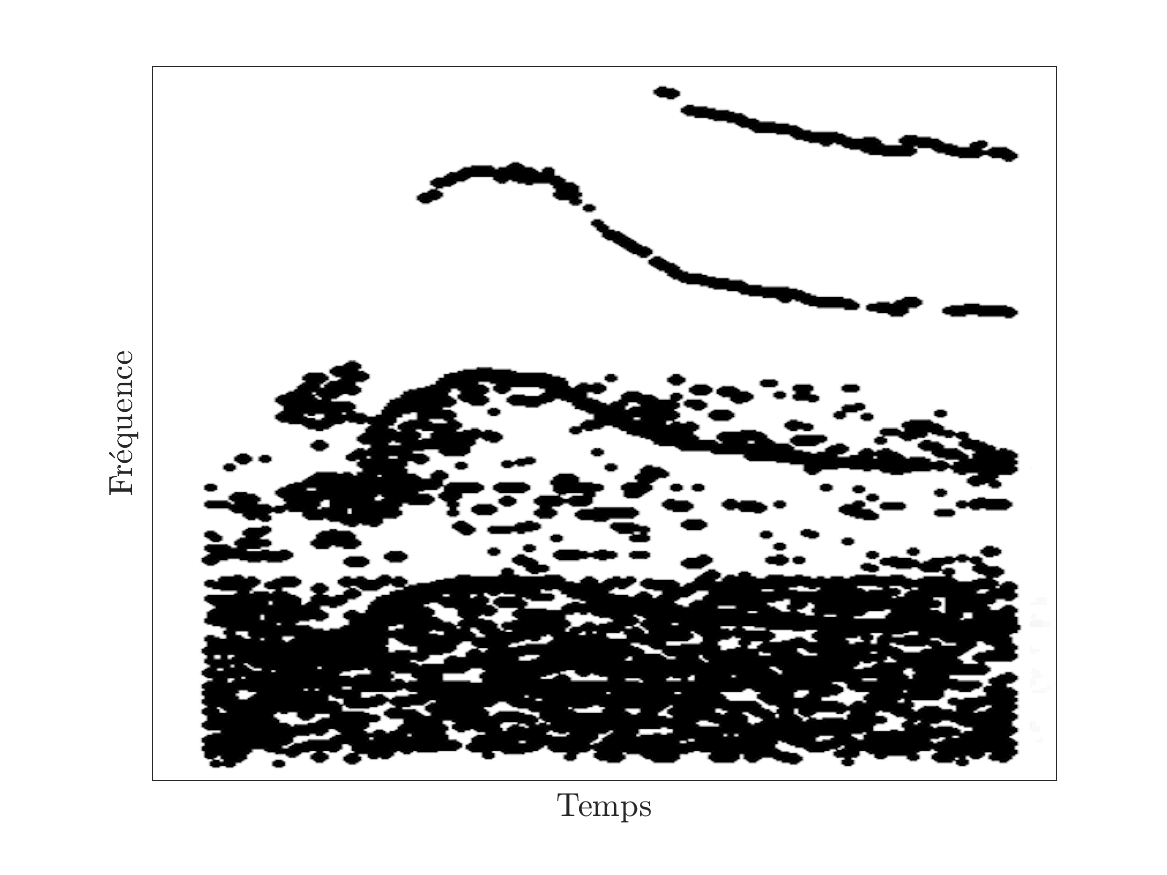
\includegraphics[width=.7\textwidth]{orcaSin}}
 \only<2>{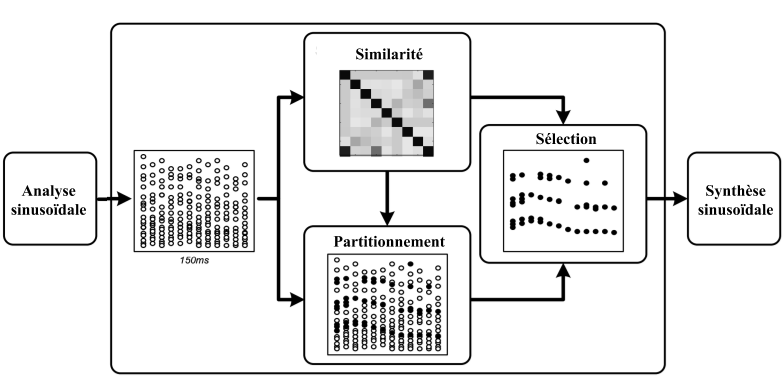
\includegraphics[width=.8\textwidth]{figures/ncutDiagramFr} \footfullcitenomarkleft{shi2000normalized}}
 \only<3>{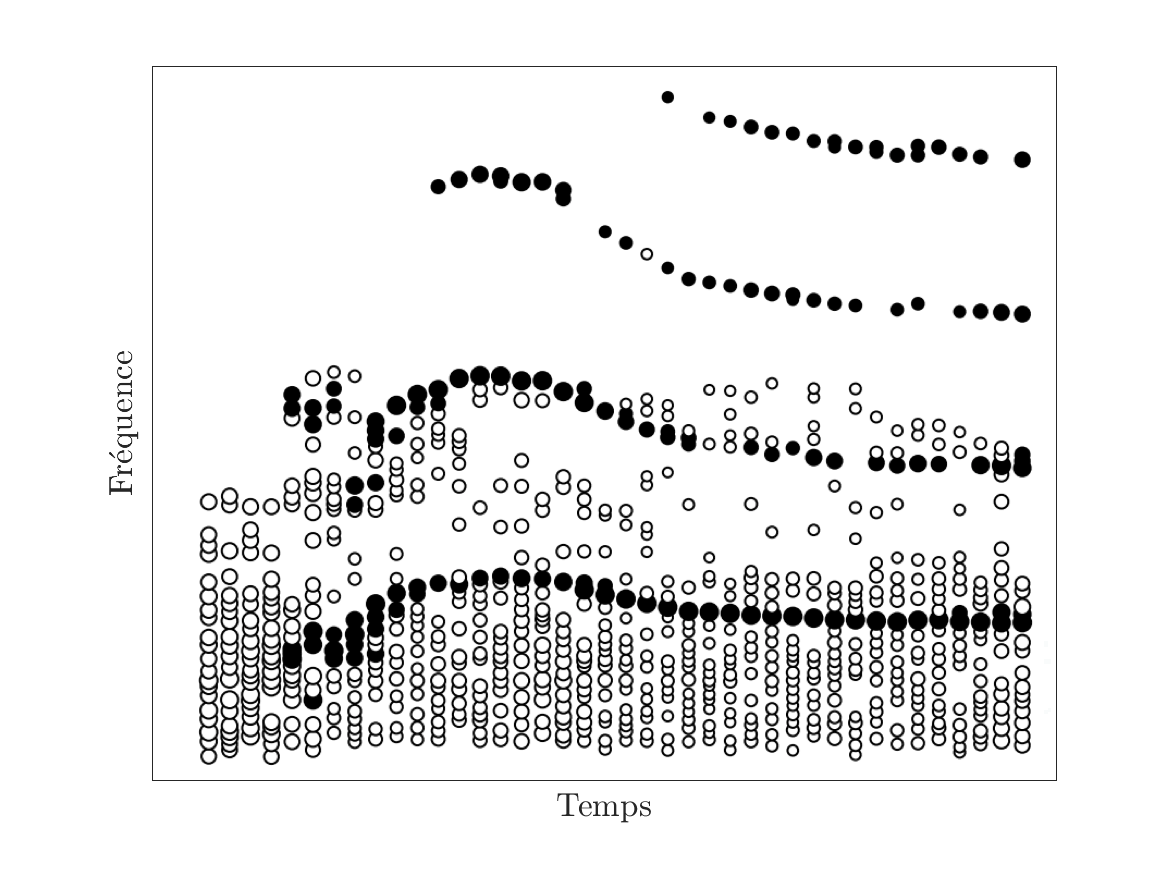
\includegraphics[width=.7\textwidth]{orcaSep}  \footfullcitenomarkleft{lagrangeTaslp08}}
\end{center}
\end{frame}



\begin{frame}{Processus ASA \og séquentiels \fg}
\begin{description}
\item[proximité] : des éléments proches les uns des autres sur le plan temps/fréquence ont tendance à être groupés ensemble
\item[similarité] : des éléments qui se ressemblent ont tendance à être groupés ensemble (timbre).
\item[...]
\end{description}
\end{frame}

\begin{frame}{Regroupement hiérarchique alterné (ANR JCJC Houle)}
\footfullcitenomarkleft{rossignol2018efficient}
\footfullcitenomarkleft{rossignolhal-01122006}
\begin{center}
   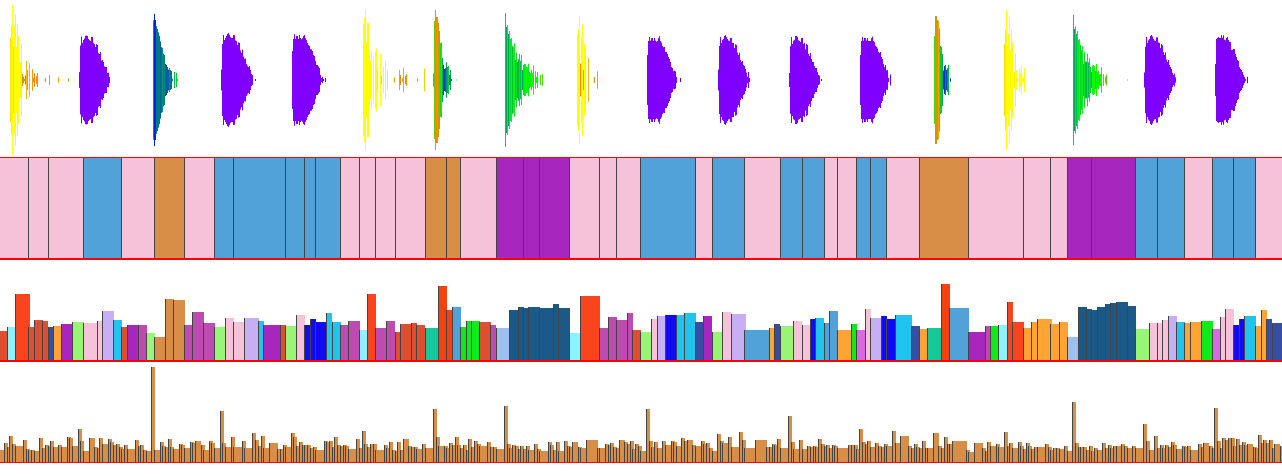
\includegraphics[width=.9\textwidth]{alc_sample}
\end{center}
\end{frame}

\begin{frame}{Approches \og algorithmiques \fg}
\begin{itemize}
\item Expression d'\textit{a priori} sous forme d'heuristiques computationnelles
\item Algorithmes de structuration non supervisés
\end{itemize}
\begin{block}{Bilan}
\begin{itemize}
\item[\textbf{+}] approches long terme : exploitation d'intervalles d'observation long
\item[\alert{\textbf{-}}] représentation court terme : problèmes de résolution
\item[\textbf{+}] pas d'apprentissage : protocole expérimental simple, interprétabilité
\item[\alert{\textbf{-}}] pas d'apprentissage : problèmes de tractabilité, problèmes d'efficience
\end{itemize}
\end{block}
\end{frame}

\section[Expérimentation]{Expérimentation en traitement du signal audio-numérique} \begin{frame}{\only<1>{\'Expérimentation}\only<2>{Contributions}}
\begin{center}
\begin{tikzpicture}[mystyle]
\matrix [column sep=10mm,row sep=5mm,ampersand replacement=\&]
{
\& \node (i4) {E};  \& \\
\node (i1) {X}; \&
\node [terminal] (i2) {$p$}; \&
\node  (i3) {Y}; \\
};
\node (box) [draw, line width=1pt, rounded corners, fit =  (i1) (i4) (i3)] {};
\begin{scope}[every path/.style=line]
  \path (i1) -- node [left] {} (i2);
  \path (i2) -- node [right] {} (i3);
\end{scope}
\end{tikzpicture}
\end{center}
\vspace{.8cm}
\only<1>{
\begin{description}
\item[$p$]: processus, traitement, prédicteur
\item[$X$]: entrée, signal, observation
\item[$Y$]: sortie, prédiction
\item[$E$]: protocole expérimental
\end{description}}
\only<2>{
\begin{description}
  \item[$X$]: plus de contrôle
  \item[$Y$]: plus de maîtrise
  \item[$E$]: plus de formalisation
\end{description}}
\end{frame}


\begin{frame}{Tâche: recherche d'information (IR)}
\begin{center}
\begin{tikzpicture}[mystyle]
\matrix [column sep=10mm,row sep=5mm,ampersand replacement=\&]
{
\node (i1) {X}; \&
\node [terminal] (i2) {$p$}; \&
\node (i3) {\alert{y}}; \\
};
\begin{scope}[every path/.style=line]
  \path (i1) -- node [left] {} (i2);
  \path (i2) -- node [left] {} (i3);
\end{scope}
\end{tikzpicture}
\end{center}
\vspace{.8cm}
\begin{description}
\item[$X$] en grande dimension
\item[$y$] en petite dimension
\end{description}
\end{frame}


\begin{frame}{Communautés}
\begin{block}{Music Information Retrieval (MIR)}
\begin{itemize}
\item 2000 - --
\item Challenge: 18 tâches  (Mirex)
\item Conference : 100 articles (Ismir)
\end{itemize}
\end{block}
\begin{block}{Detection and Classification of
Acoustic Scenes and Events (DCASE)}
\begin{itemize}
\item 2013 - --
\item Challenge: 7 tâches
\item Workshop: 50 articles
\end{itemize}
\end{block}
\end{frame}

\begin{frame}{Tâche: recherche d'information (IR)}
\begin{center}
\begin{tikzpicture}[mystyle]
\matrix [column sep=10mm,row sep=5mm,ampersand replacement=\&]
{
\node (i1) {X}; \&
\node [terminal] (i2) {$P$}; \&
\node [terminal] (i3) {$C$}; \&
\node (i4) {\alert<1>{y}}; \\
};
\begin{scope}[every path/.style=line]
  \path (i1) -- node [left] {} (i2);
\path (i2) -- node [above] {$L$} (i3); \path (i3) -- node [right] {} (i4);
\end{scope}
\end{tikzpicture}
\end{center}
\vspace{.8cm}
\begin{description}
\item[$X$] en grande dimension
\item[$L$] ..., aussi finalement
\item[but]: $X_j=D(X_i)$, $L_j=d(L_i) \text{ ssi } y_j=y_i$
\item[$D$]: grande déformation
\item[$d$]: petite déformation
\end{description}
\end{frame}

\begin{frame}{Propriétés de $L$}
  \begin{center}
  \begin{tikzpicture}[mystyle]
  \matrix [column sep=10mm,row sep=5mm,ampersand replacement=\&]
  {
  \node (i1) {X}; \&
  \node [terminal] (i2) {$P$}; \&
  \node [terminal] (i3) {$C$}; \&
  \node (i4) {\alert<1>{y}}; \\
  };
  \begin{scope}[every path/.style=line]
    \path (i1) -- node [left] {} (i2);
  \path (i2) -- node [above] {$L$} (i3); \path (i3) -- node [right] {} (i4);
  \end{scope}
  \end{tikzpicture}
  \end{center}
  \vspace{.8cm}
  \begin{block}{Guidé par les données $X$}
    \begin{itemize}
    \item invariance: translation, ...
    \item stabilité: étirement, ...
    \end{itemize}
  \end{block}
  \begin{block}{Guidé par la tâche $y$}
$$ |L_i-L_j| < |L_i-L_k| \text{ ssi } y_i=y_j \forall k | y_k \neq y_i $$
  \end{block}
\end{frame}


\begin{frame}{IR en audio}
\begin{center}
\begin{tikzpicture}[mystyle]
\matrix [column sep=10mm,row sep=5mm,ampersand replacement=\&]
{
\node (i1) {X}; \&
\node [terminal] (i2) {$P$}; \&
\node [terminal] (i3) {$C$}; \&
\node (i4) {y}; \\
};
\begin{scope}[every path/.style=line]
  \path (i1) -- node [left] {} (i2);
  \path (i2) -- node [above] {  } (i3);
  \path (i3) -- node [right] {} (i4);
\end{scope}
\end{tikzpicture}
\end{center}
\vspace{.8cm}
\begin{description}
\item[$P$]: module de \og perception \fg
\begin{itemize}
    \item plusieurs TFCT à résolutions différentes
    \item réseaux convolutionnels profonds
\end{itemize}
\item[$C$]: module de \og cognition \fg
\begin{itemize}
    \item réseaux neuronaux profonds totalement connectés
    \item fusion
\end{itemize}
\end{description}
\end{frame}


\begin{frame}{Challenges en IR}
\begin{center}
\begin{tikzpicture}[mystyle]
\matrix [column sep=10mm,row sep=5mm,ampersand replacement=\&]
{
\& \node (i4) {E};  \& \\
\node (i1) {\alert<5>{X}}; \&
\visible<2->{\node [terminal] (i2) {\only<2>{$p_1$}\only<3>{$p_2$}\only<4>{$p_n$}\only<5>{$p$}}; \&
\node  (i3) {y};} \\
};
\node (box) [draw, line width=1pt, rounded corners, fit =  (i1) (i4) (i3)] {};
\visible<2->{
\begin{scope}[every path/.style=line]
  \path (i1) -- node [left] {} (i2);
  \path (i2) -- node [right] {} (i3);
\end{scope}}
\end{tikzpicture}
\end{center}
\vspace{.8cm}
\visible<4->{
\begin{itemize}
\item Alternative à l'approche \og mon outil, mon jeu de données, ma métrique \fg
\item Spécification de l'expérimentation  \og clés en main \fg
\item biais de conception du protocole assumés collectivement
\end{itemize}
}
\end{frame}

\begin{frame}{Design de Challenge}
\begin{block}{Organisation d'une tâche DCASE (2013, 2016)}
\begin{itemize}
\item Tâche de détection d'évènements
\item corpus de scènes sonores simulées
\item sons isolés enregistrés
\item contrôle de haut niveau sur la composition de la scène
\end{itemize}
\end{block}\footfullcitenomarkleft{stowellhal-01253912} \footfullcitenomarkleft{mesa}
\end{frame}

\begin{frame}{Challenges en crise ?}
\begin{itemize}
    \item cauchemard des métriques
    \item \og la fin justifie les moyens \fg
\end{itemize}
\vspace{.8cm}
\begin{center}
\og Faites quelque chose d'intéressant !! \fg \\
\og ... de scientifique !! \fg \\
\hfill \textit{panel DCASE 2018}
\end{center}
\vspace{.8cm}
$\hookrightarrow{}$ placer l'effort sur un questionnement plutôt que sur la démonstration d'un outil
\end{frame}

\begin{frame}{Approche  \og psychologie expérimentale \fg}
\begin{itemize}
\item formulation d'une hypothèse : le degré de polyphonie impacte les algorithmes de détection d'évènement sonores
\item production de corpus avec un degré variable de polyphonie
\item choix d'un protocole expérimental adapté
\item les algorithmes sont considérés comme des sujets et leurs concepteurs ne sont pas informés de la typologie du corpus
\item analyse des résultats
\end{itemize} \footfullcitenomarkleft{lafayhal-01111381}
\end{frame}

\begin{frame}{Que prédire ?}
\begin{center}
  \begin{tikzpicture}[mystyle]
  \matrix [column sep=10mm,row sep=5mm,ampersand replacement=\&]
  {
  \& \node (i4) {E};  \& \\
  \node (i1) {X}; \&
  \node [terminal] (i2) {p}; \&
  \node  (i3) {\alert{y}}; \\
  };
  \node (box) [draw, line width=1pt, rounded corners, fit =  (i1) (i4) (i3)] {};
  \begin{scope}[every path/.style=line]
    \path (i1) -- node [left] {} (i2);
    \path (i2) -- node [right] {} (i3);
  \end{scope}
  \end{tikzpicture}
\end{center}
\vspace{.8cm}
\begin{itemize}
\item interface riche avec d'autres communautés
\item nécessité d'alignement des vocabulaires et des temporalités
\end{itemize}
\end{frame}

\begin{frame}{Caractérisation des environnements sonores urbains (ANR CENSE)}
  \begin{minipage}{.5\columnwidth}
    \begin{itemize}
    \item les qualifiants perceptifs de haut niveau comme l'agrément sont corrélés au temps de présence perçu des sources
    \item prédiction de ces valeurs perceptives par des approches neuronales
    \end{itemize}
  \end{minipage}
  \begin{minipage}{.4\columnwidth}
    \begin{center}
    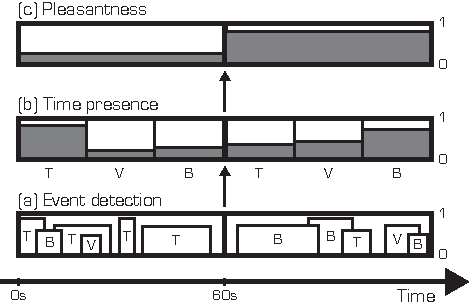
\includegraphics[width=\columnwidth]{figures/block} \\
    \end{center}
  \end{minipage}
\footfullcitenomarkleft{gontierActa}
\end{frame}

\begin{frame}{Projet de recherche avec le Conservatoire National de Musique et de Danse de Paris (CNSMDP)}
\begin{itemize}
\item Recherche par similarité dans des corpus de modes de jeux étendus
\item Confrontation d'un modèle computationnel de perception à des jugements experts
\item L'opérateur de diffusion d'ondelettes apporte d'excellents résultats
\end{itemize}
\begin{table}
\small
    \centering
{\footnotesize
\begin{tabular}{c|ccccc}
 joint (1s) + lmnn & -lmnn & (25 ms) &  séparable & mfcc & \\
      \hline
 $96\% \pm 2$ & $93\% \pm 3$ & $91\% \pm 4$ & $91\% \pm 4$ & $82\% \pm 7$ & ($aP@5$)\\
\end{tabular}
}
\end{table}
\footfullcitenomarkleft{lostanlenJasmp}
\end{frame}

\begin{frame}{ExpLanes}
  \begin{center}
    \only<1>{
  \begin{tikzpicture}[mystyle]
  \matrix [column sep=10mm,row sep=5mm,ampersand replacement=\&]
  {
  \& \node (i4) {\alert{E}};  \& \\
  \node (i1) {X}; \&
  \node [terminal] (i2) {p}; \&
  \node  (i3) {y}; \\
  };
  \node (box) [draw, line width=1pt, rounded corners, fit =  (i1) (i4) (i3)] {};
  \begin{scope}[every path/.style=line]
    \path (i1) -- node [left] {} (i2);
    \path (i2) -- node [right] {} (i3);
  \end{scope}
\end{tikzpicture}}
\only<2>{  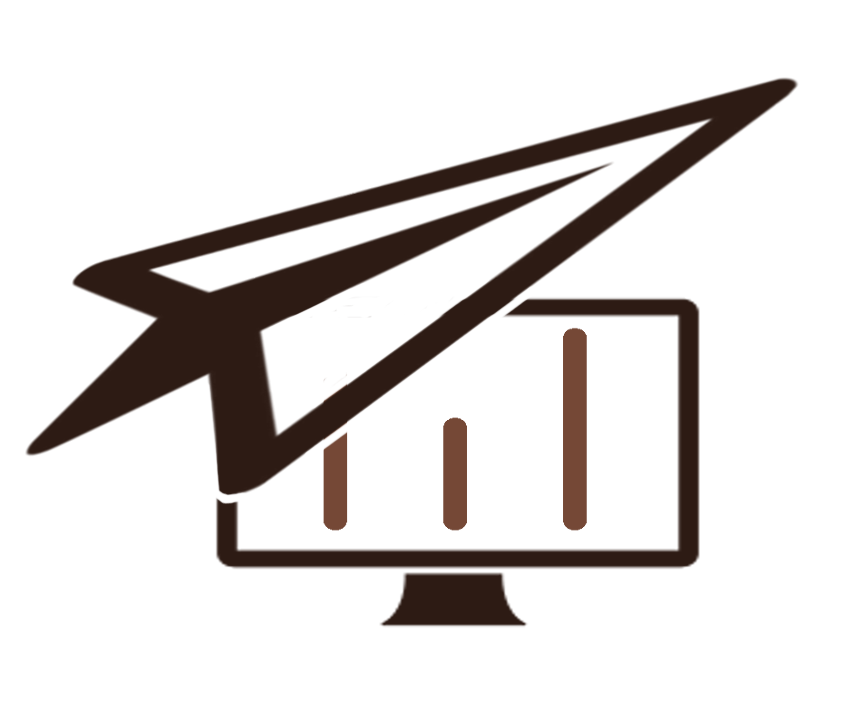
\includegraphics[width=.3\columnwidth]{figures/logoExplanes} \\
   \url{http://mathieulagrange.github.io/expLanes}}
  \end{center}
  \vspace{.8cm}
ExpLanes, un environnement logiciel qui facilite:
\begin{enumerate}
  \item la gestion des calculs
  \item le traitement des résultats
  \item la reproducibilité
\end{enumerate}
\end{frame}

\begin{frame}{ExpLanes}

  \begin{center}
  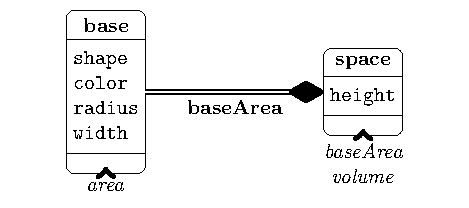
\includegraphics[width=\columnwidth]{figures/factors} \\
  \tiny  \url{https://mathieulagrange.github.io/paperBandwidthExtensionCnn/demo}
  \end{center}
\footfullcitenomarkleft{lagrange2019bandwidth}
\end{frame}

% E
% reproducibilité
% donoho
% protocoles expérimentaux assez canonique
% explanes
% extension de bande
% demonstration
\begin{frame}{Approches étudiées}
\begin{center}
\begin{tikzpicture}[mystyle]
\matrix [column sep=10mm,row sep=5mm,ampersand replacement=\&]
{
\& \node (i4) {\alert{E}};  \& \\
\node (i1) {\alert{X}}; \&
\node [terminal] (i2) {p}; \&
\node  (i3) {\alert{y}}; \\
};
\node (box) [draw, line width=1pt, rounded corners, fit =  (i1) (i4) (i3)] {};
\begin{scope}[every path/.style=line]
  \path (i1) -- node [left] {} (i2);
  \path (i2) -- node [right] {} (i3);
\end{scope}
\end{tikzpicture}
\end{center}
\vspace{.8cm}
\begin{description}
\item[$X$] plus de contrôle : données simulées
\item[$y$] plus de maîtrise : collaboration avec les communautés expertes
\item[$E$] plus de formalisation : développement d'explanes
\end{description}
\end{frame}

\section[Projet]{Projet de recherche} 
\begin{frame}{Problématiques en traitement du signal audionumérique}
\begin{center}
\begin{tikzpicture}[mystyle]
\matrix [column sep=10mm,row sep=5mm,ampersand replacement=\&]
{
\node (i1) {\only<1-2>{Son}\only<3-4>{\alert{contrôleurs}}}; \&
\node [terminal] (i2) {p}; \&
\node  (i3) {\only<2>{label}\only<1>{Son}\only<3-4>{\alert{Son}}}; \\
};
\begin{scope}[every path/.style=line]
  \path (i1) -- node [left] {} (i2);
  \path (i2) -- node [right] {} (i3);
\end{scope}
\end{tikzpicture}
\end{center}
\vspace{.8cm}\only<1-3>{
\begin{description}
\item<1>[X-Y]: codage, séparation de sources, \structure{extension de bande}, inpainting, ...
\item<2>[X-y]: recherche d'information
\item<3>[x-Y]: synthèse
\end{description}}
\only<4>{
\begin{itemize}
\item attrait personnel pour l'inouï
\item challenge
\item en prise avec les avancées actuelles en apprentissage non supervisé
\end{itemize}}
\end{frame}

\begin{frame}{Requis}
\begin{description}
  \item[fidélité]: ne pas produire d'artefacts audibles
  \item[expressivité]: mécanismes de manipulation simples produisant une modification cohérente de la perception du signal résultant
  \item[versatilité]: les conditions de fidélité et d'expressivité sont remplies pour tout signal d'intérêt pour une tâche donnée
\end{description}
\end{frame}

\begin{frame}{\only<1>{Existant}\only<2>{Objectif}}
\begin{tabular}{cc}
\begin{tikzpicture}[scale=0.8, label distance=1.5mm]
  \coordinate[label=below:Fidélité]  (A) at (0,0);
  \coordinate[label=below:Versatilité] (B) at (4,0);
  \coordinate[label=above:Expressivité] (C) at (2,3.464);
  \draw [line width=1.5pt] (A) -- (B) -- (C) -- cycle;
  \draw [black, fill=black, line width=1.5pt] (2,.3) circle [radius=.1 cm]; % raw
  \draw [olive, fill=olive, line width=1.5pt] (1.8,.8) circle [radius=.1 cm]; % spec
  \draw [brown, fill=brown, line width=1.5pt] (2.4,.6) circle [radius=.1 cm]; % wavelets
  \draw [cyan, fill=cyan, line width=1.5pt] (1.6,1.2) circle [radius=.1 cm]; % sct
  \draw [blue, fill=blue, line width=1.5pt] (1.4,1.8) circle [radius=.1 cm]; % slt
  \draw [magenta, fill=magenta, line width=1.5pt] (1.9,2.6) circle [radius=.1 cm]; % modal
  \only<2>{\draw [black, line width=1.5pt] (2.4,1.8) circle [radius=.2 cm];} % modal
  \end{tikzpicture}

 &

  \begin{tabular}{cl}
    \tikz\draw[black,fill=black] (0,0) circle (.1 cm); & Forme d'onde \\
    \tikz\draw[olive,fill=olive] (0,0) circle (.1 cm); & Spectrogramme \\
    \tikz\draw[brown,fill=brown] (0,0) circle (.1 cm); & Ondelettes \\
    \tikz\draw[cyan,fill=cyan] (0,0) circle (.1 cm); & Sinusoïdes à court terme \\
    \tikz\draw[blue,fill=blue] (0,0) circle (.1 cm); & Sinusoïdes à long terme \\
    \tikz\draw[magenta,fill=magenta] (0,0) circle (.1 cm); & Approches modales
  \end{tabular}
  \end{tabular}
\end{frame}

\begin{frame}{Challenges en traitement du signal}
\newcommand{\blackdot}{\tikz\draw[black,fill=black] (0,0) circle (.1 cm);}
\centering
\begin{block}{La synthèse en audio nécessite d'approcher les challenges suivants}
  \begin{tabular}{c|ccc}
    & fidélité & versatililité & expressivité  \\
  %  \hline
  multirésolution & \blackdot  & \blackdot & \\
  causalité & \blackdot  &  & \blackdot \\
  non linéarité & \blackdot  & \blackdot & \\
  dimensionalité réduite &  & &  \blackdot \\
  contrôle lent &  & &  \blackdot
  \end{tabular}
\end{block}
\end{frame}

\begin{frame}{Schéma fonctionnel}
  \begin{center}
  \structure{IR} \\  \vspace{.2cm}  \begin{tikzpicture}[mystyle]
      \matrix [column sep=10mm,row sep=5mm,ampersand replacement=\&]
      {
      \node (i1) {Son}; \&
      \node [terminal] (i2) {$P$}; \&
      \node [terminal] (i3) {$C$}; \&
      \node (i4) {label}; \\
      };
      \begin{scope}[every path/.style=line]
        \path (i1) -- node [left] {} (i2);
      \path (i2) -- node [above] {$L$} (i3); \path (i3) -- node [right] {} (i4);
      \end{scope}
      \end{tikzpicture}
 \vspace{.4cm} \\  \structure{Synthèse} \\ \vspace{.2cm}
      \begin{tikzpicture}[mystyle]
      \matrix [column sep=10mm,row sep=5mm,ampersand replacement=\&]
      {
      \node (i1) {contrôleurs}; \&
      \node [terminal] (i2) {$c$ \only<2>{\alert{??}}}; \&
      \node [terminal] (i3) {$V$ \only<2>{\alert{??}}}; \&
      \node (i4) {Son}; \\
      };
      \begin{scope}[every path/.style=line]
        \path (i1) -- node [left] {} (i2);
      \path (i2) -- node [above] {$L$} (i3); \path (i3) -- node [right] {} (i4);
      \end{scope}
      \end{tikzpicture}
      \end{center}
      \begin{description}
        \item[$P$]: invariance / stabilité
        \item[$c$]: conditionneur
        \item[$V$]: vocodeur ($P^{-1}$)

      \end{description}
\end{frame}


\begin{frame}{Recherche en cours}
\begin{description}
\item[Vocodeur]: inversion de descripteurs pour la synthèse de scènes sonores respectueuses de la vie privée (Félix Gontier)
\item[conditionneur]: conception interactive en design sonore (Tom Souaille)
\end{description}
\end{frame}

\begin{frame}{Problèmes ouverts}
\begin{itemize}
  \item Spécification des objectifs
  \begin{itemize}
  \item mesure quantitatives de qualité perceptuelles
  \item fonctions de coût perceptivement motivées
  \end{itemize}
\item Synthèse audio neuronale
\begin{itemize}
  \item modèles génératifs adversaires
\item approches basées échantillons
\end{itemize}
\item Opérateur de diffusion d'ondelettes
\begin{itemize}
\item pour le conditionnement
\item pour la synthèse par inversion
\end{itemize}
\end{itemize}
\end{frame}

%


\begin{frame}{Réseau}
\begin{block}{Local}
\begin{itemize}
\item Jean-François Petiot (LS2N)
\item Arnaud Can, Judicaël Picaut, ... (UMRAE, IFSTTAR)
\end{itemize}
\end{block}
\begin{block}{National}
\begin{itemize}
\item Nicolas Misdariis (IRCAM)
\item Catherine Lavandier (U. Cergy)
\end{itemize}
\end{block}
\begin{block}{International}
\begin{itemize}
\item Emmanouil Benetos (QMUL, UK)
\item Vincent Lostanlen (NYU, US)
\item Joakim Andèn (Flatiron Institute, US)
\end{itemize}
\end{block}
\end{frame}

\begin{frame}{\only<1,9>{Un travail en inter-disciplinarité} \only<2>{France Télécom R\&D (2001-04)}\only<3>{Bx (2004-06)}\only<4>{Uvic (2006-07)}\only<5>{McGill (2007-08)}\only<6>{Télécom (2008-09)}\only<7>{Ircam (2009-13)}\only<8>{Ls2n (2013-19)}}
  \begin{tikzpicture}[mystyle]
      \matrix [column sep=20mm,row sep=20mm,ampersand replacement=\&]
      {
      \node (imu) {Musicologie}; \&
      \node  (ipe) {Perception}; \&
      \node  (id) {Design}; \\
      \node [align=center](ima) {Maths\\ Appli}; \&
      \node [terminal,align=center] (its) {Traitement \\du signal\\ audio}; \&
      \node  (iph) {Physique}; \\
      \node  {}; \&
      \node  (ii) {Informatique}; \&
      \node   {}; \\
      };
      \begin{scope}[every path/.style=line, font=\scriptsize]
        \path (ima) -- node [above] {\only<7>{A. Cont}\only<6>{R. Badeau} \only<1,8>{E. Benetos}} (its);
            \path (ima) -- node [below] {\only<6>{G. Richard}\only<1>{J. Andèn}} (its);
        \path (imu) -- node [right] {\only<3>{M. Robine} \only<8>{G. Lafay} \only<1>{V. Lostanlen}} (its);
        \path (iph) -- node [above] {\only<2>{JB. Rault} \only<5>{P. Depalle} \only<7>{A. Roebel}\only<8>{JR. Gloaguen}  \only<1>{J. Picaut}} (its);
        \path (iph) -- node [below] {\only<5>{G. Scavone} } (its);
        \path (ii) -- node [right] {\only<2-3>{S. Marchand}\only<4>{G. Tzanetakis}\only<6>{S. Essid}} (its);
        \path [align=left] (id) -- node [right] {\only<1,8>{\hspace{.3cm}JF. Petiot}\only<1,7>{\\ N. Misdariis}} (its);
        \path [align=left] (ipe) -- node [right] {\only<5>{C. Guastavino}\only<1>{C. Lavandier}\only<1,8>{\\ A. Can}} (its);
        \end{scope}
      \end{tikzpicture}
\end{frame}



    % \begin{frame}{Approche}
    % \begin{center}
    %  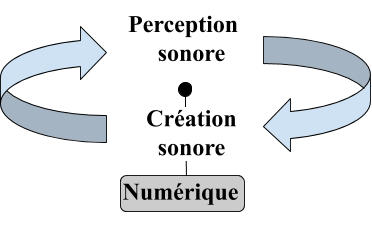
\includegraphics[width=.6\columnwidth]{longTerme}
    % \end{center}
    % \begin{description}
    % \item[comprendre] : mesure et qualification de l'environnement sonore et de sa perception
    % \item[innover] :
    % \begin{itemize}
    % \item Andy Hildebrand (Autotune)
    % \item Xavier Serra (Vocaloïd)
    % \end{itemize}
    % \end{description}
    % \end{frame}

% \begin{frame}{Déplacements US}
% \begin{block}{Côte ouest}
% \begin{itemize}
% \item \structure{Jesse Engel}, magenta, Google brain (SFB)
% \item Justin Salamon, audio research group, Adobe research (SFB)
% \end{itemize}
% \end{block}
% \begin{block}{Côte est}
% \begin{itemize}
% \item Juan Pablo Bello, music and audio research group, NYU (NY)
% \item Mounya Elhilali, Laboratory for Computational Audio Perception, Johns Hopkins University (Baltimore)
% \end{itemize}
% \end{block}
% \end{frame}

% \begin{frame}{Contributions}
% \small
% Publications
% \begin{itemize}
% \item \fullcite{lagrangeTaslp06}
% \item \fullcite{lagrangeTaslp08}
% \item \fullcite{lafayhal-01111381}
% \end{itemize}
% Logiciels
% \begin{itemize}
% \item \fullcite{explanes}
% \item \fullcite{simscene}
% \end{itemize}
% \end{frame}


\end{document}
